\chapter{Analisis}
\label{chap:analisis}
Pada bab ini dijelaskan mengenai deskripsi perangkat lunak,  analisis data histori KIRI , analisis perangkat lunak, dan analisis \textit{heat map} dan \textit{marker clustering} menggunakan  \textit{Google Maps Javascript API}.

\section{Deskripsi Perangkat Lunak}
\label{sec:deskripsiPL}
Pada skripsi ini akan dibangun aplikasi yang bertujuan untuk menemukan pola dengan tool visualisasi. Aplikasi ini akan menggunakan data histori perangkat lunak KIRI sebagai sumber data. Aplikasi ini akan dibangun menggunakan \textit{tools} nodejs dan akan mengimplementasikan \textit{google maps javascript api} sebagai tool untuk melakukan visualisasi data. Beberapa fitur yang dirancang dalam perangkat lunak ini:
\begin{itemize}
\item Perangkat lunak dapat memfilter data berdasarkan atribut \textit{start/finish}.
\item Perangkat lunak dapat memfilter data berdasarkan atribut waktu.
\item Perangkat lunak dapat memfilter data berdasarkan atribut hari.
\item Perangkat lunak dapat menampilkan data dalam bentuk \textit{heat map}
\item Perangkat lunak dapat menampilkan data dalam bentuk \textit{marker clustering}.
\end{itemize}
Perangkat lunak ini akan melukan filter data dan memproses data histori kiri dan akan menampilkan data tersebut kedalam bentuk \textit{heat map} dan \textit{marker clustering} untuk mendapatkan pola-pola tertentu berdasarkan data histori tersebut. Berikut ini adalah gambaran alur komunikasi perangkat lunak yang akan dibuat:

\begin{figure}[H]
	\centering  
	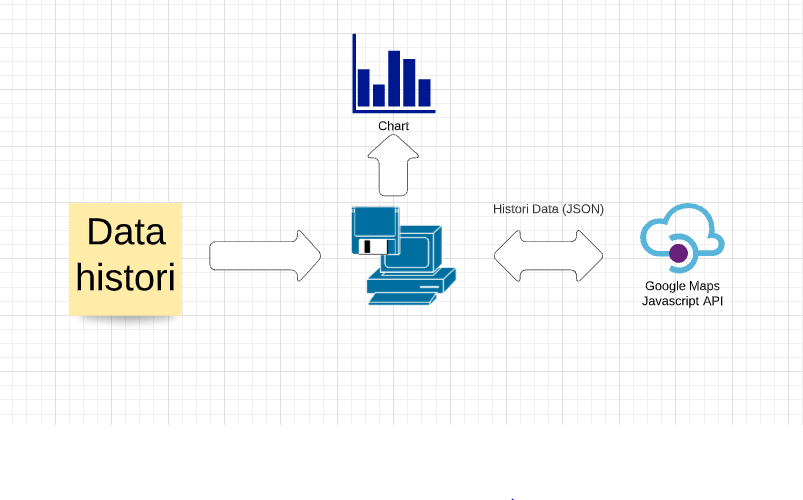
\includegraphics[scale=0.55]{Gambar/software-flow.PNG}  
	\caption[Alur Komunikasi]{Alur Komunikasi} 
	\label{fig:alurKomunikasi} 
\end{figure} 

\begin{enumerate}
\item Perangkat lunak akan mengolah data histori kiri sesuai dengan input yang diberikan.
\item Data yang sudah diolah  akan diubah kedalam format \textit{JSON}.
\item Data yang sudah diolah akan digunakan oleh \textit{Google Maps Javascript API} untuk dapat dilakukan visualisasi data.
\item Perangkat lunak akan memvisualisasikan data kedalam bentuk \textit{heat map} dan \textit{marker clustering}.

\end{enumerate}

\section{Analisis Data Histori KIRI}
Perangkat lunak yang akan menggunakan data histori KIRI sebagai sumber data untuk melakukan visualisasi data. Data histori KIRI memiliki format \textit{csv}. Data histori KIRI memiliki lima atribut yaitu:
\begin{itemize}
    \item LogId
    Id unik  sebagai penanda satu record didalam data histori KIRI.
    \item APIKey
     atribut api key yang digunakan ketika melakukan perintah pada perangkat lunak KIRI.
    \item Timestamp (UTC)
    atribut untuk mencatat waktu perintah dilakukan format berbentuk \textit{timestamp}.
    \item Action
    jenis action yang dilakukan user pada saat menggunakan perangkat lunak KIRI. Terdapat empat nilai action pada data histori KIRI yakni:
    \begin{itemize}
        \item \textit{PAGELOAD}.
        \item \textit{SEARCHPLACE}.
        \item \textit{WIDGETLOAD}.
        \item \textit{FINDROUTE}.
    \end{itemize}
    \item AdditionalData atribut yang digunakan untuk mencatat informasi tambahan berdasarkan action yang dipilih. Nilai pada additionaldata akan bergantung pada action yang dipilih:
    \begin{itemize}
        \item jika action bernilai \textit{PAGELOAD} maka additionaldata akan bernilai ip dari pengakses.
        \item jika action bernilai \textit{SEARCHPLACE} maka additionaldata akan bernlai keyword yang dituliskan oleh pengakses.
        \item jika action bernilai \textit{FINDROUTE} maka additionaldata akan bernilai posisi tempat dan tujuan dalam bentuk langtitude dan longtitude  yang dicari oleh pengakses.
        \item jika action bernilai \textit{WIDGETLOAD} maka additionaldata akan bernilai alamat url dari penyedia widget.
    \end{itemize}
\end{itemize}

Perangkat lunak akan mengubah format data histori KIRI dari bentuk  \textit{csv} menjadi \textit{json} dimana format atribut json akan berupa:
\begin{verbatim}
    [{"timestamp":"2014-1-2:0:11",
    "start":"-6.8972513,107.6385574",
    "finish":"-6.91358,107.62718"},
    {"timestamp":"2014-1-2:0:13",
    "start":"-6.8972513,107.6385574",
    "finish":"-6.91358,107.62718"}]
\end{verbatim}
agar dapat diparsing menggunakan \textit{google maps javascript api}.

\section{Analisis Perangkat Lunak}
\subsection{Analisis Kebutuhan Perangkat Lunak}
Berdasarkan latar belakang, rumusan masalah, dan tujuan maka dapat didefinisikan kebutuhan - kebutuhan perangkat lunak visualisasi data histori KIRI sebagi berikut:
\begin{itemize}
    \item Data histori KIRI
    Aplikasi dapat melakukan proses filter pada data histori dan menggunakan data histori KIRI untuk dapat divisualisasikan oleh karena itu diperlukan raw data histori KIRI.
    
    \item Google Maps Javascript API
    Aplikasi dapat melakukan visualisasi data menggunakan \textit{heat map} dan \textit{marker clustering} yang merupakan fitur dari \textit{google maps javascript api}.
    
\end{itemize}
\section{Use Case Diagram}
Interaksi antara pengguna dengan perangkat lunak yang dibangun pada skripsi ini digambarkan pada diagram \textit{use case} dan skenario berikut ini
\begin{figure}[H]
	\centering  
	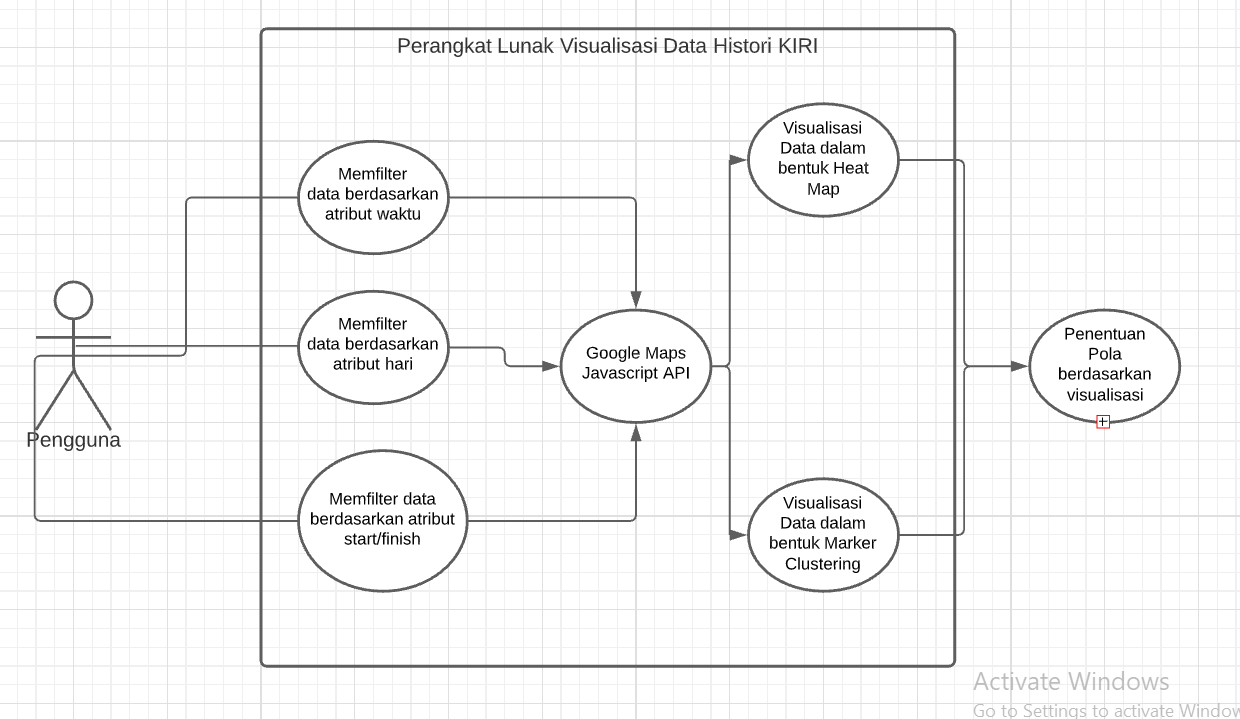
\includegraphics[scale=0.55]{Gambar/usecase.PNG}  
	\caption[Use Case]
	\label{fig:usecase} 
\end{figure} 
\subsection{\textit{Use Case} Skenario}
Setiap fungsi yang ada pada diagram \textit{use case} dijelaskan dengan skenario untuk memberi gambaran interaksi pengguna dengan sistem.
\begin{table}[H]
    \centering
    \caption{Tabel Skenario Memfilter Data Berdasarkan Atribut Waktu}
    \begin{tabular}{|p{3cm}|p{10cm}|}
    \hline
        Nama & Memfilter Data Berdasarkan Atribut Waktu.\\
    \hline
    \hline
        Deskripsi & Melakukan filter data berdasarkan input waktu yang diberikan oleh pengguna \\
    \hline
        Aktor & Pengguna \\
    \hline
        Pre-kondisi & Aplikasi sudah dijalankan dan sudah dapat mengolah raw data histori KIRI.\\
    \hline
        Alur Skenario Utama & 
        \begin{enumerate}
            \item Sistem memuat aplikasi.
            \item Sistem menampilkan data.
            \item Pengguna memfilter data berdasarkan waktu".
            \item Sistem melakukan proses filtering menggunakan atribut waktu.
            \item Sistem memvisualisasikan data yang telah difilter oleh pengguna.
        \end{enumerate}\\
    \hline
    \end{tabular}
    \label{tab:skenario1}
\end{table}

\begin{table}[H]
    \centering
    \caption{Tabel Skenario Memfilter Data Berdasarkan Atribut Hari}
    \begin{tabular}{|p{3cm}|p{10cm}|}
    \hline
        Nama & Memfilter Data Berdasarkan Atribut Hari.\\
    \hline
    \hline
        Deskripsi &  Melakukan filter data berdasarkan input Hari yang diberikan oleh pengguna. \\
    \hline
        Aktor & Pengguna \\
    \hline
        Pre-kondisi & Aplikasi sudah dijalankan dan sudah dapat mengolah raw data histori KIRI.\\
    \hline
        Alur Skenario Utama & 
        \begin{enumerate}
            \item Sistem memuat aplikasi.
            \item Sistem menampilkan data.
            \item Pengguna memfilter data berdasarkan hari".
            \item Sistem melakukan proses filtering menggunakan atribut hari.
            \item Sistem memvisualisasikan data yang telah difilter oleh pengguna.
        \end{enumerate}\\
    \hline
    \end{tabular}
    \label{tab:skenario1}
\end{table}

\begin{table}[H]
    \centering
    \caption{Tabel Skenario Memfilter Data Berdasarkan Atribut Start/Finish}
    \begin{tabular}{|p{3cm}|p{10cm}|}
    \hline
        Nama & Memfilter Data Berdasarkan Atribut  Start/Finish.\\
    \hline
    \hline
        Deskripsi &  Melakukan filter data berdasarkan input  Start/Finish yang diberikan oleh pengguna. \\
    \hline
        Aktor & Pengguna \\
    \hline
        Pre-kondisi & Aplikasi sudah dijalankan dan sudah dapat mengolah raw data histori KIRI.\\
    \hline
        Alur Skenario Utama & 
        \begin{enumerate}
            \item Sistem memuat aplikasi.
            \item Sistem menampilkan data.
            \item Pengguna memfilter data berdasarkan hari".
            \item Sistem melakukan proses filtering menggunakan atribut  Start/Finish.
            \item Sistem memvisualisasikan data yang telah difilter oleh pengguna.
        \end{enumerate}\\
    \hline
    \end{tabular}
    \label{tab:skenario1}
\end{table}

\begin{table}[H]
    \centering
    \caption{Tabel Skenario Penggunaan Google Maps Javascript API}
    \begin{tabular}{|p{3cm}|p{10cm}|}
    \hline
        Nama & M Penggunaan Google Maps Javascript API.\\
    \hline
    \hline
        Deskripsi &  Menggunakan Google Maps Javascript API untuk memvisualisasikan data histori kiri \\
    \hline
        Aktor & Pengguna \\
    \hline
        Pre-kondisi & Aplikasi sudah berhasil memproses data berdasarkan filter dari pengguna\\
    \hline
        Alur Skenario Utama & 
        \begin{enumerate}
            \item Sistem menerima input filter dari pengguna.
            \item Sistem mengubah data kedalam format JSON.
            \item Sistem menggunakan Google Maps Javascript API".
            \item Sistem memvisualisasikan data yang telah difilter oleh pengguna.
        \end{enumerate}\\
    \hline
    \end{tabular}
    \label{tab:skenario1}
\end{table}